\documentclass[11pt,a4paper]{article}
\usepackage[utf8]{inputenc}
\usepackage[T1]{fontenc}
\usepackage[brazil]{babel}
\usepackage{lmodern}
\usepackage[margin=2cm]{geometry}
\usepackage{amsmath,amssymb}
\usepackage{booktabs}
\usepackage{graphicx}
\usepackage{hyperref}
\usepackage{xcolor}
\usepackage{titlesec}
\usepackage{tabularx}
\usepackage{enumitem}
\usepackage{float}
\usepackage{array}
\renewcommand{\tabularxcolumn}[1]{>{\raggedright\arraybackslash}p{#1}}

\hypersetup{
    colorlinks=true,
    linkcolor=blue!70!black,
    citecolor=blue!70!black,
    urlcolor=blue!70!black
}

\titleformat{\section}{\large\bfseries}{\thesection.}{0.5em}{}
\titleformat{\subsection}{\normalsize\bfseries}{\thesubsection.}{0.5em}{}
\titlespacing*{\section}{0pt}{1.2ex plus 0.5ex minus .2ex}{0.6ex}
\titlespacing*{\subsection}{0pt}{1.0ex plus 0.4ex minus .2ex}{0.4ex}

\setlength{\parskip}{0.45em}
\setlength{\parindent}{0pt}
\setlist{itemsep=0.15em,topsep=0.3em}
\newcommand{\Mx}[1]{\textit{#1}}

\begin{document}

\begin{center}
    {\Large \textbf{Relatório de Status do TCC}} \\[0.25em]
    {\normalsize Avaliação das Explicações SHAP em Redes Neurais Profundas para Classificação de Arritmias Cardíacas em ECG} \\[0.2em]
    \textbf{Aluno:} Arthur Santos de Oliveira (RA: 156297) \quad \textbf{Orientador:} Prof.\ Dr.\ Luis Augusto Martins Pereira \\[0.15em]
    \textbf{Data:} 11/11/2026 \quad \textbf{Repositório:} \url{https://github.com/Arthur-so/shap-ecg-arrhythmia}
\end{center}
\vspace{-0.6em}
\hrule
\vspace{0.5em}

\section{Situação geral}
Os experimentos estão \textbf{concluídos} e a redação começou: os capítulos de \textbf{Materiais e Métodos} e de \textbf{Resultados e Discussão} já têm uma versão completa (24 páginas, 14 figuras), no formato de TCC do curso. Faltam a Introdução, a Fundamentação Teórica, os Trabalhos Relacionados e a Conclusão. A pergunta do trabalho é se a qualidade das explicações GradientSHAP, medida por métricas quantitativas, acompanha o desempenho (F1) do modelo em cada classe de arritmia.

\section{O que está pronto}
\begin{itemize}
\item \textbf{Modelo:} ResNet34-1D no CPSC2018 (9 classes, multirrótulo), F1-macro de \textbf{0,819} no teste, próximo de Zhang et al.\ (2021), 0,813, com F1 por classe também próximo (AF e BRD acima de 0,92; STE a pior, 0,596).
\item \textbf{Explicações:} 622 mapas GradientSHAP (predições corretas do teste), com referência balanceada de 36 ECGs (4 por classe) e 200 sorteios por mapa.
\item \textbf{Regiões do batimento:} cada mapa é resumido em 36 valores (figura na Seção~4) (12 derivações × pré-QRS, QRS e ST-T), a partir dos picos R. Os limites foram justificados clinicamente e por precedentes (Wagner et al., 2024; Gumpfer et al., 2026; Turbé et al., 2023) e testados em 9 combinações alternativas, sem mudar as pontas da ordem das classes.
\item \textbf{Métricas:} sete métricas reimplementadas por regiões, com a implementação conferida contra o artigo original de cada uma: \Mx{Faithfulness Correlation}, \Mx{Faithfulness Estimate}, \Mx{Max/Avg-Sensitivity}, \Mx{Consistency}, \Mx{Complexity}, \Mx{Random Logit} e eMPRT. As comparações entre mapas são lidas em relação ao \textbf{piso}, a variação do próprio GradientSHAP entre sementes (0,18).
\item \textbf{Revisão da literatura:} 12 fichamentos completos e 36 curtos (9 deles das referências de apoio da Metodologia), guia de leitura e relatório da revisão.
\end{itemize}

\section{O que cada métrica avalia e resultados}
Todas as métricas usam o mapa resumido nas 36 regiões. ``Retirar'' uma região é trocar todos os seus pontos por zero (a média da derivação) e ver quanto cai a saída (logit) da classe explicada. Quando uma métrica compara dois mapas, a distância é lida em relação ao \textbf{piso}: a distância entre dois mapas do mesmo ECG gerados com sementes diferentes (média de 0,18, numa escala de 0 a 2). Só uma distância acima do piso indica uma mudança maior que a variação do próprio GradientSHAP.

\begin{itemize}
\item \textbf{\Mx{Faithfulness Correlation}} (fidelidade; Bhatt et al., 2020). \textit{Avalia} se as regiões que o mapa diz serem importantes são as que mais influenciam o modelo. \textit{Como:} sorteiam-se 50 conjuntos de 9 regiões; para cada um, compara-se a soma das atribuições com a queda da saída ao retirá-lo, pela correlação de Pearson (1 = o mapa prevê perfeitamente a queda). \textit{Resultado:} 0,60 global, comparável aos 0,41 a 0,63 da família SHAP em ECG (Suh et al., 2024). BRD (0,75) no topo; SNR (0,45) e STD (0,47) embaixo.

\item \textbf{\Mx{Faithfulness Estimate}} (fidelidade; Alvarez-Melis e Jaakkola, 2018). \textit{Avalia} o mesmo, região por região. \textit{Como:} cada uma das 36 regiões é retirada sozinha, e a sua atribuição é correlacionada com a queda que ela causa. \textit{Resultado:} 0,61 global, com a mesma ordem: BRD (0,78) e BRE (0,70) no alto, STD e SNR (0,49) embaixo.

\item \textbf{\Mx{Max/Avg-Sensitivity}} (robustez; Yeh et al., 2019; Bhatt et al., 2020). \textit{Avalia} se a explicação muda pouco quando o ECG muda pouco. \textit{Como:} soma-se um ruído pequeno ao ECG (10 vezes), o mapa é refeito com a mesma semente, e mede-se a maior (Max) e a média (Avg) das distâncias ao mapa original. \textit{Resultado:} 0,045 e 0,036, cerca de \textbf{4 vezes menores que o piso}: as explicações são robustas, e o que mais as faz variar é o sorteio do próprio método. A ordem das classes repete a da fidelidade.

\item \textbf{\Mx{Consistency}} (Dasgupta et al., 2022). \textit{Avalia} se ECGs que recebem a mesma explicação recebem a mesma predição. \textit{Como:} cada mapa é resumido pelas suas 2 regiões principais (com o sinal); para cada mapa, calcula-se a fração dos outros mapas com o mesmo resumo que explicam a mesma classe, comparada com o valor esperado ao acaso. \textit{Resultado:} 0,455 global, acima do acaso em todas as classes; é a métrica mais próxima do F1 (AF, BRD e IAVB no alto; CAP e STE embaixo).

\item \textbf{\Mx{Complexity}} (Bhatt et al., 2020). \textit{Avalia} se a importância está concentrada em poucas regiões, o que facilita a leitura. \textit{Como:} calcula-se a entropia das frações de importância e a converte no número efetivo de regiões (de 1, tudo numa região, a 36, tudo igual). \textit{Resultado:} 24 de 36 regiões: os mapas são espalhados. BRD, AF e IAVB são os mais concentrados; STD, o mais espalhado.

\item \textbf{\Mx{Random Logit}} (randomização; Sixt et al., 2020). \textit{Avalia} se o mapa muda quando se pergunta por outra classe. \textit{Por quê:} um método de explicação pode simplesmente destacar o que chama atenção no ECG (por exemplo, os QRS, que são os picos mais altos), qualquer que seja a classe pedida. Nesse caso, o mapa que ``explica o BRD'' e o que ``explica a STE'' seriam iguais, e o mapa não diria nada sobre a decisão do modelo. \textit{Como:} num ECG com BRD, por exemplo, gera-se o mapa da classe BRD e o mapa de uma classe que o ECG não tem (como STE), com a mesma semente, para que só a classe mude. Compara-se a distância entre os dois (0 = mapas iguais; 2 = opostos). Se a distância ficasse perto do piso, a explicação não dependeria da classe. \textit{Resultado:} distância média de 1,60, cerca de 10 vezes o piso, e todos os 4\,886 pares ficam acima do piso: os mapas são específicos da classe explicada. AF tem os mapas mais específicos e STE, os menos, o que acompanha o F1.

\item \textbf{eMPRT} (randomização; Hedström et al., 2023). \textit{Avalia} se o mapa depende do que o modelo aprendeu. \textit{Por quê:} se um mapa sai praticamente igual de uma rede treinada e de uma rede que não aprendeu nada, ele não explica o modelo; descreve só o ECG. \textit{Como:} sorteiam-se de novo todos os pesos da rede, o que apaga o aprendizado, e refaz-se o mapa do mesmo ECG com a mesma semente. O critério do artigo é que o mapa do modelo aleatório fique \textbf{mais espalhado} (maior entropia, $q > 0$), porque não haveria mais regiões que o modelo ``usa''. \textit{Resultado:} o critério falha ($q = -0{,}015$): o mapa do modelo aleatório fica até mais concentrado, quase sempre nos QRS (as 2 regiões principais são de QRS em 88\% dos mapas, contra 42\% no modelo treinado). \textit{Por que isso é esperado:} o mapa do GradientSHAP é o gradiente multiplicado por (ECG $-$ referência). Num modelo aleatório, o gradiente não tem estrutura, mas o segundo fator continua lá, e ele é maior justamente onde o ECG tem os maiores valores, os picos do QRS. O mapa passa a reproduzir a forma do próprio ECG, como Adebayo et al.\ (2018) observaram para os métodos do tipo gradiente × entrada (a estrutura da entrada permanece; muda o sinal das atribuições). A entropia não detecta isso, mas as distâncias detectam: o mapa do modelo aleatório fica a 8,7 vezes o piso do mapa treinado, e a região principal coincide em só 5\% dos casos. O mapa depende, portanto, do modelo; o eMPRT é usado como teste de sanidade, e não para comparar classes.
\end{itemize}

\section{Principais resultados}
\begin{table}[H]\centering\small
{\small Relação de cada grupo de métricas com o F1 por classe (comparação descritiva, por posição das classes).}\par\vspace{0.3em}
\begin{tabularx}{\linewidth}{>{\raggedright\arraybackslash}p{4.6cm}>{\raggedright\arraybackslash}p{2.3cm}X}
\toprule
\textbf{Métricas} & \textbf{Valor global} & \textbf{Relação com o F1} \\
\midrule
\Mx{Consistency}, \Mx{Random Logit} & 0,455; 1,60 & Acompanham o F1 nas pontas: AF, BRD e IAVB no alto; CAP e STE embaixo. \\ \addlinespace
\Mx{Faithfulness Correlation} e \Mx{Estimate} & 0,60; 0,61 & Não acompanham: seguem o tipo de evidência (QRS: BRD, BRE, CVP no alto; ritmo e ST: SNR, AF, CAP, STD embaixo). \\ \addlinespace
\Mx{Max/Avg-Sensitivity} & 0,045; 0,036 & Mesma ordem da fidelidade; ambas 4 vezes menores que o piso. \\ \addlinespace
\Mx{Complexity} & 24 de 36 regiões & Parcial: as três mais concentradas são as três de maior F1. \\ \addlinespace
eMPRT & $q = -0{,}015$ & Falha no critério de entropia, mas o mapa depende do modelo (distância 8,7 vezes o piso); usado como teste de sanidade. \\
\bottomrule
\end{tabularx}
\end{table}
\vspace{-0.6em}
\textbf{Conclusão parcial:} a resposta \textbf{depende da propriedade medida}. As métricas que envolvem a decisão do modelo entre classes acompanham o F1; as de fidelidade e robustez acompanham a amplitude e o tipo da região diagnóstica de cada classe, o que concorda com Gumpfer et al.\ (2026) e Baer et al.\ (2025a, 2025b). Não se encontrou, na revisão, trabalho que relacione diretamente a qualidade das explicações com o F1 por classe.

\begin{figure}[H]\centering
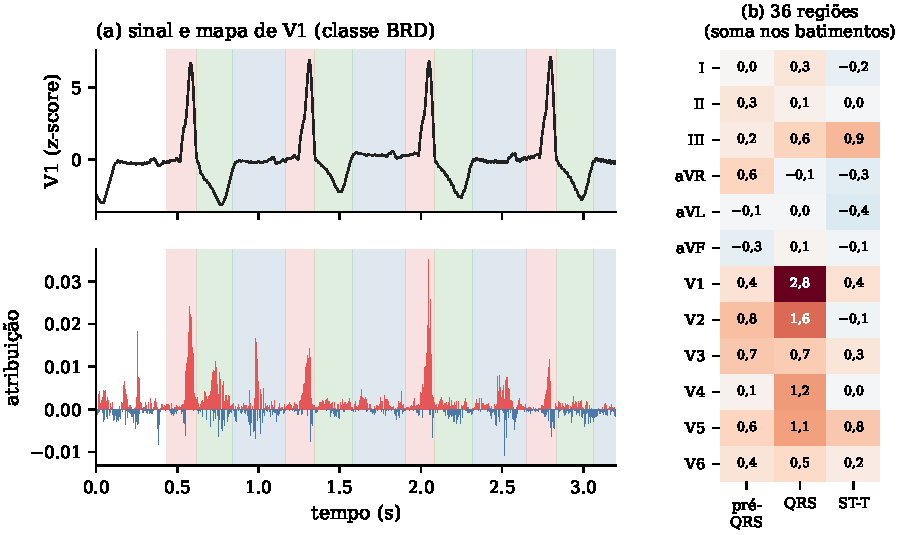
\includegraphics[width=0.82\linewidth]{figs/agregacao.pdf}\\[-0.2em]
{\small Exemplo (ECG de BRD): o mapa de V1 e o vetor das 36 regiões; a região principal é o QRS de V1, onde o BRD é reconhecido clinicamente.}
\end{figure}
\vspace{-0.8em}

\end{document}
